	\documentclass[11pt, a4paper, spanish]{article}

\usepackage{alltt}

%%%%%%%%%% COMIENZO DEL PREAMBULO %%%%%%%%%%

%Info sobre este documento
\author{Mart\'n Cammi}
\title{Trabajo Pr\'actico de Algoritmos y Estucturas de datos III}

%\usepackage{infostyle}                                                  % provee un look & feel similar a un documento Word
\usepackage[top=2.5cm, bottom=2.5cm, left=2.5cm, right=2.5cm]{geometry}  % m\'argenes
\usepackage[ansinew]{inputenc}                                           % permite que los acentos del estilo \'a\'e\'i\'o\'u salgan joya
\usepackage[spanish, activeacute]{babel}                                 % idioma espaniol, acentos f\'aciles y deletreo de palabras
\usepackage{indentfirst}                                                 % permite indentar un parrafo a mano
\usepackage{caratula}                                                    % incluye caratula est\'andar
\usepackage{graphicx}                                                    % permite insertar gr\'aficos
\usepackage{color}                                                       % permite el uso de colores en el documento
\usepackage[pdfcreator={TexLive!, LaTeX2e con TeXnicCenter},
			pdfauthor={Grupo: "1"},
			pdftitle={Algoritmos III - Trabajo Pr\'actico 2},
			pdfsubject={Trabajo Pr\'actico 1},
			pdfkeywords={Prismas, Esferas, Punto de corte, puente, pizza},
			pdfstartview=FitH,            % Fits the width of the page to the window
			bookmarksnumbered,            % los bookmarks numerados se ven mejor...
			colorlinks,                   % links con bellos colores
			linkcolor=magenta]            % permite cambiar el color de los links
			{hyperref}                    % Permite jugar con algunas cosas que aparecer\'an en el PDF final

%RESTAURAR
\usepackage{algorithm}							% Permite tabular un codigo
\usepackage{algorithmic}
%\floatname{algorithm}{Algoritmo}
\renewcommand{\listalgorithmname}{Lista de algoritmos}
\renewcommand{\algorithmicrequire}{\textbf{Entrada:}}
\renewcommand{\algorithmicensure}{\textbf{Salida:}}
\renewcommand{\algorithmicend}{\textbf{fin}}
\renewcommand{\algorithmicif}{\textbf{si}}
\renewcommand{\algorithmicthen}{\textbf{entonces}}
\renewcommand{\algorithmicelse}{\textbf{si no}}
\renewcommand{\algorithmicelsif}{\algorithmicelse,\ \algorithmicif}
\renewcommand{\algorithmicendif}{\algorithmicend\ \algorithmicif}
\renewcommand{\algorithmicfor}{\textbf{para}}
\renewcommand{\algorithmicforall}{\textbf{para todo}}
\renewcommand{\algorithmicdo}{\textbf{hacer}}
\renewcommand{\algorithmicendfor}{\algorithmicend\ \algorithmicfor}
\renewcommand{\algorithmicwhile}{\textbf{mientras}}
\renewcommand{\algorithmicendwhile}{\algorithmicend\ \algorithmicwhile}
\renewcommand{\algorithmicloop}{\textbf{repetir}}
\renewcommand{\algorithmicendloop}{\algorithmicend\ \algorithmicloop}
\renewcommand{\algorithmicrepeat}{\textbf{repetir}}
\renewcommand{\algorithmicuntil}{\textbf{hasta que}}
\renewcommand{\algorithmicprint}{\textbf{imprimir}} 
\renewcommand{\algorithmicreturn}{\textbf{devolver}} 
\renewcommand{\algorithmictrue}{\textbf{cierto }} 
\renewcommand{\algorithmicfalse}{\textbf{falso }} 
 % mi archivo de traducci\'on			

%\selectlanguage{spanish}

%\selectlanguage{spanish}
\linespread{1.3}                    % interlineado equivalente al 1.5 l\'ineas de Word...
\pagestyle{myheadings}              %encabezado personalizable con \markboth{}{}
\markboth{}{Algoritmos III  - Trabajo Pr\'actico 2 - Cammi, Garbi, Kretschmayer}
\headsep = 30pt                     % separaci\'on entre encabezado y comienzo del p\'arrafo

%\addtolength{\oddsidemargin}{-2cm}	% configuracion IDEAL!!!
%\addtolength{\textwidth}{4cm}
%\addtolength{\textheight}{2cm}

% macro 'todo' para To-Do's
\def\todo#1{\textcolor{red}{#1}}

% Macro 'borde' para un texto con borde
\newsavebox{\fmbox}
\newenvironment{borde}[1]
{\begin{lrbox}{\fmbox}\begin{minipage}{#1}}
{\end{minipage}\end{lrbox}\fbox{\usebox{\fmbox}}\\[10pt]}

%%%%%%%%%% FIN DEL PREAMBULO %%%%%%%%%%

\begin{document}

\materia{Algoritmos y Estucturas de datos III}
\submateria{Segundo Cuatrimestre de 2011}
\titulo{Trabajo Pr\'actico 2}
\subtitulo{Problema1: Esferas vs Prismas. \ \ \ \ \ \ \ \ \ \ \ \ \ \ \ \ \ \ \ \ \ \ \ \ \ \ \ \ \ \ \ \ \ \ \  Problema2: Puntos de corte y puentes. \ \ \ \ \ \ \ \ \ \ \ \ \ \ \ \ \ \ Problema3: M\'as Pizza entre amigos.}
\grupo{Grupo: `1'}
\integrante{Cammi, Mart\'in}{676/02}{martincammi@gmail.com}
\integrante{Garbi, Sebasti\'an}{179/05}{garbyseba@gmail.com}
\integrante{Kretschmayer, Daniel}{310/99}{daniak@gmail.com}

\maketitle

\thispagestyle{empty}

\tableofcontents

\newpage


\textbf{Ejecuci\'on del TP}
\label{sec:ejecucion}

	\subsection{Lenguaje utilizado}
		
		El lenguaje utilizado para el trabajo pr\'actico ha sido \emph{Java}, compilando con la versi\'on 1.5 de la Virtual Machine.
		
		El trabajo se acompa\~{n}a con los fuentes de la soluci\'on que puede importarse en IDE de Eclipse o ejecutarse desde l\'inea de comandos.

	\subsection{Como ejecutar el TP}
	
	\textbf{\underline{Desde l\'inea de comandos}}
	\begin{itemize}
			\item{Posicionarse en el directorio Algo3Tp2}
			\item{Copiar all\'i el archivo de entrada para el problema i, por ejemplo Ej1.in}
			\item{Ejecutar el comando: \emph{java -cp ./bin problema1.Ej1}}
	\end{itemize}
	Esto generar\'a el archivo Ej1.out con la soluci\'on en el mismo directorio Algo3Tp2.

	\textbf{\underline{Desde el Eclipse}}
	
	Primero importaremos el proyecto:	
	
	\begin{itemize}
			\item{Seleccionar File $\Rightarrow$ Import.}
			\item{Seleccionar General $\Rightarrow$ Existing Projects into Workspace $\Rightarrow$ Next.}
			\item{Seleccionar el directorio llamado Algo3Tp2.}
			\item{Finish.}
	\end{itemize}
	
	Desde la vista de \textbf{Package Explorer} bajo el paquete \textbf{src} aparecer\'an tres paquetes m�s y dentro de cada uno de ellos los siguientes archivos de java:\\

	\begin{center}
		%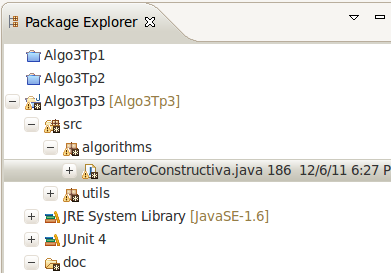
\includegraphics[scale=0.65]{others/packageExplorer.png}\\
		COLOCAR IMAGEN CORRECTA
	\end{center}

\newpage

	Para ejecutar un problema:

	\begin{itemize}
			\item{Posicionarse en el directorio Algo3Tp2}
			\item{Copiar en el directorio Algo3Tp2 el archivo de entrada para el problema i, por ejemplo Ej1.in}
			\item{Con bot\'on derecho Run As $\Rightarrow$ Java Application. Se ejecutar\'a el problema seleccionado.}
	\end{itemize}
	Esto generar\'a el archivo Ej1.out con la soluci\'on en el mismo directorio Algo3Tp2.

\newpage

% Conviene poner las secciones como diferentes archivos,
% sobre todo cuando se trabaja en equipo.
% Es m\'as f\'acil para sincronizar mediante control de versiones.
%\input{Introducci\'on}

% Problema1
\section{Problema1: Esferas vs Prismas}
\label{sec:problema1}
	\subsection{Introducci\'on}

	La guerra contra los prismas se ha declarado y debemos ayudar a las esferas a ganarla.\\
	La batalla se libra en un campo minado de prismas, agrupados uno al lado del otro en forma de una grilla de $l x a$. Cada prisma tienen una altura y un rango y una esfera puede destruir un prisma golpe\'andolo en la cabeza y continuar destruyendo otros prismas si estos est\'an contiguos y tienen menor altura que el que ya destruy'o. El nivel de destrucci\'on es la suma de todos los rangos de los prismas ca\'idos en combate.\\
	 Nuestro objetivo es idear un algoritmo para que las esferas puedan producir la mayor cantidad de destrucci\'on posible.\\
	
	\subsection{Explicaci\'on de la soluci\'on}
	
	El objetivo es lograr encontrar un camino que parta desde un prisma y vaya recorriendo prismas adyacentes de menor altura y que este camino tenga el rango o nivel de destrucci\'on m\'aximo posible.

	La idea del algoritmo es recorrer estos caminos al rev\'es. Comenzaremos recorriendo cada prisma de la grilla y para cada uno de ellos haremos recursi'on preguntando si pudo haber venido de alg\'un otro mayor, preguntando a sus 4 vecinos. Si alguno de ellos es mayor que \'el significa que un camino de destrucci\'on pudo haber venido de ese prisma y volveremos recursivamente a preguntarle a ese prisma de donde pudo haber venido. De esta manera iremos recorriendo los prismas hasta que encontremos un prisma mayor a todos sus vecinos y no podamos continuar. Este prisma ser\'a el caso base, es decir el prisma el inicial para uno de los caminos que pueda tomar la esfera. 

A medida que vamos recorriendo estos caminos en la recursi\'on iremos al mismo tiempo calculando el \emph{Nivel de Destrucci\'on} y en base a \'el guardaremos para cada prisma un \emph{de donde vino} para poder luego identificar el camino de mayor destrucci\'on.

En el siguiente ejemplo se muestra el recorrido del algoritmo, supondemos para simplificar este ejemplo que el rango de cada prisma es igual a su altura, as\'i el prisma de altura 1 tiene un rango igual a 1.

	\begin{center}
		\includegraphics[scale=0.40]{p1/PrismasyEsferas1.png}\\
	\end{center}

En el ejemplo figuran 4 prismas, comenzaremos calculando la mayor destrucci\'on del el prisma 1.

	\begin{center}
		\includegraphics[scale=0.40]{p1/PrismasyEsferas2.png}\\
	\end{center}

Los prismas de mayor altura adyacentes al prisma 1 son dos, el que est\'a a su derecha y el que est\'a abajo. El algoritmo recorrer\'a a sus vecinos en sentido de las agujas del reloj comenzando por el vecino superior. En este caso el Prisma 1 no tiene vecino superior por lo que continuar\'a por su vecino de la derecha.

	\begin{center}
		\includegraphics[scale=0.40]{p1/PrismasyEsferas3.png}\\
	\end{center}

Ahora situados en el prisma 2, recorreremos todos los vecinos con altura mayor que \'el, el \'unico es el prisma 3. (el gui\'on indica de que prisma se vino desde la recursi\'on)

	\begin{center}
		\includegraphics[scale=0.40]{p1/PrismasyEsferas4.png}\\
	\end{center}

Hemos llegado al prisma 3 el cual no tiene vecinos mayores que \'el con lo cual formar\'a el inicio de un camino de destrucci\'on.

	\begin{center}
		\includegraphics[scale=0.40]{p1/PrismasyEsferas5.png}\\
	\end{center}

Le asignamos el rango del mismo prisma que es tres (lo indicaremos en la parte inferior derecha de cada prisma) ya que no pudo haber venido de otro prisma.

	\begin{center}
		\includegraphics[scale=0.40]{p1/PrismasyEsferas6.png}\\
	\end{center}

Retornamos entonces en la recursi\'on volviendo al prisma 2 y preguntamos si la destrucci\'on acumulada de 2 supera la de su vecino reci\'en calculado 3. Como 2 todav\'ia no tiene asignado destrucci\'on acumulada lo actualizaremos con la de 3 mas el valor de su rango, es decir 5.


	\begin{center}
		\includegraphics[scale=0.40]{p1/PrismasyEsferas6-5.png}\\
	\end{center}

Retornamos entonces en la recursi\'on volviendo al prisma 1 y preguntamos si la destrucci\'on acumulada de 1 supera la de su vecino reci\'en calculado 2. Como 1 todav\'ia no tiene asignado destrucci\'on acumulada lo actualizaremos con la de 2 mas el valor de su rango, es decir 6.\\

	\begin{center}
		\includegraphics[scale=0.40]{p1/PrismasyEsferas7.png}\\
	\end{center}

Al mismo tiempo hemos retornado en la recursi\'on de 1 habiendo obtenido el valor de destrucci\'on de su vecino derecho, nos falta ver el nivel de destrucci\'on de su vecino de abajo.

	\begin{center}
		\includegraphics[scale=0.40]{p1/PrismasyEsferas8.png}\\
	\end{center}

Ahora situados en el prisma 2 (de abajo), recorreremos todos los vecinos con altura mayor que \'el, el \'unico es el prisma 3 nuevamente. 

	\begin{center}
		\includegraphics[scale=0.40]{p1/PrismasyEsferas9.png}\\
	\end{center}

Como de iteraciones anteriores el prisma 3 ya tiene calculado su nivel de destrucci\'on, no entraremos en recursi\'on para el prisma 3 nuevamente, sino que simplemente preguntamos si la destrucci\'on acumulada de 2 supera la de su vecino 3 ya calculado. Como 2 todav\'ia no tiene asignado destrucci\'on acumulada lo actualizaremos con la de 3 mas el valor de su rango, es decir 5.

	\begin{center}
		\includegraphics[scale=0.40]{p1/PrismasyEsferas10.png}\\
	\end{center}

Finalmente hemos vuelto de la recursi\'on del prisma 1 y ya no quedan vecinos por recorrer.
Sin embargo pueden haber quedado prismas sin visitar que no hayan sido alcanzables desde la recursi\'on del prisma 1. Es por eso que asi como hicimos con el prisma 1 recorreremos todos los prismas de la grilla para asegurarnos que no quede ninguno sin visitar pero con la salvedad de que no entraremos en la recursi\'on en ellos si su nivel de destrucci\'on ya fue calculado por alg�n otro camino previo. Esto nos evitar\'a hacer recursi\'on innecesariamente.\\

En el ejemplo, como ya para todos los prismas se han logrado calcular sus niveles de destrucci\'on, si bien los recorreremos para verificarlo no haremos recursi\'on en ninguno de ellos nuevamente.


Cabe aclarar que para poder calcular el camino final debemos guardar un par de datos.\\
Cada vez que actualizamos el nivel de destrucci\'on de un prisma, guardamos tambi\'en el vecino del cual obtuvo mayor nivel para luego poder identificar el camino de mayor destrucci\'on. Tambi\'en guardamos el prisma que haya acumulado el mayor nivel para luego comenzar de \'el a reconstruir el camino.

	\begin{center}
		\includegraphics[scale=0.40]{p1/PrismasyEsferas11.png}\\
	\end{center}

En el ejemplo el prisma que acumul\'o mayor destrucci\'on fue el 1 con un nivel de 6. El 1 obtuvo parte de ese nivel de parte del prisma 2 de su derecha (se guard\'o que venia del 2). El prisma 2 a su vez qued\'o con un nivel de 5 y obtuvo parte de \'el del prisma 3 (se guard\'o que venia del 3).
El prisma 3 obtuvo su nivel de \'el mismo, ya que sus vecinos tenian todos altura menor con lo cual se guard\'o que venia de \'el mismo (Esto nos ayudar\'a al rearmar el camino saber cuando terminar de recorrer, es decir, cuando un prisma haya venido de si mismo.\\

El mayor camino de destrucci\'on entonces con un nivel de 6 ser\'a:\\

	\begin{center}
		\includegraphics[scale=0.40]{p1/PrismasyEsferas12.png}\\
	\end{center}

El algoritmo trabaja realizando una mezcla entre backtracking volviendo recursivamente para obtener la mejor soluci\'on y programaci\'on din\'amica por la cual una vez calculado el nivel de un prisma lo guarda en una variable de acceso constante para no realizar c\'alculos innecesarios.

\newpage
	
\subsection{Pseudo-c\'odigo}

\begin{algorithm}
\caption{calcularCaminoDeMaximaDestruccion}
\label{alg1}
\begin{algorithmic}

	\FOR {Cada prisma de la matriz}
		\IF {tiene guardado el nivel de destrucci\'on acumulado}
			\RETURN nivel de destrucci\'on acumulado del prisma
		\ELSE
			\FOR {Cada vecino de mayor altura}
				\STATE calcularMaximaDestruccion(vecino)
			\ENDFOR				
			vecinoConMaximaDestrucci\'on = calcular cual de los anteriores es el vecino de m\'axima destrucci\'on

			\IF {prisma.destruccionAcumulada > vecinoConMaximaDestrucci\'on.destrucci\'onAcumulada}
				\STATE prisma.destrucci\'onAcumulada = prisma.rango
				\STATE prisma.desdeDondeVino = prisma.INICIO
			\ELSE
				\STATE prisma.destrucci\'onAcumulada = prisma.rango + vecinoConMaximaDestrucci\'on.destrucci\'onAcumulada
				\STATE prisma.desdeDondeVino = vecinoConMaximaDestrucci\'on
			\ENDIF
		\ENDIF

		\IF{vecinoConMaximaDestrucci\'on > maximo}
			\STATE maximo = vecinoConMaximaDestrucci\'on
		\ENDIF
	\ENDFOR

	\WHILE {!maximo.desdeDondeVino != prisma.INICIo}
		\STATE agrego el prisma a una lista para luego devolverla
	\ENDWHILE
	 
\end{algorithmic}
\end{algorithm}	


\subsection{Modelo Elegido}

	El modelo elegido ser\'a el \emph{Modelo Uniforme} porque las operaciones son escencialmente comparaciones y sumas que podemos asumir de orden constante sin que por ello afecte la complejidad del algoritmo.
\newpage
	
\subsection{Complejidad}

	El algoritmo tendr\'a que recorrer todos los elemento de la grilla por lo menos una vez esto da un orden de $O(l \cdot a)$.\\

	Por otro lado tenemos que tener en cuenta las llamadas recursivas, habr\'a una por cada vez que un prisma visite a otro prisma superior a \'el (recordemos que el algoritmo busca los caminos de forma inversa). 

	\begin{center}
		\includegraphics[scale=0.30]{p1/PrismasyEsferasUnidasPorAristas.png}\\
	\end{center}

Los prismas est\'an agrupados en una grilla y se recorren a trav\'es de alguno de sus posibles cuatro vecinos adyacentes. Podemos imaginarnos dicha grilla como un grafo en donde cada arista representa un pasaje recursivo de un prima a uno de mayor altura. Por la forma de recorrer del algoritmo pasaremos una sola vez por cada una de estas ``aristas`` ya que en caso de tener el nivel precalculado no deberemos hacer recursi\'on.\\

De esta forma para cada prisma el algoritmo tendr\'a como posibilidades para recursi\'on todas las fechas salientes. En el ejemplo anterior las flechas corresponden a recursiones reales sobre los prismas. En cualquier grilla el \'unico caso en que una de estas aristas no sea recorrida es que ambos prismas tengan la misma altura. En cualquier otro caso o bien un prisma vecino a otro lo llamar\'a en una recursi\'on o bien su vecino lo llamar\'a a el.

	\begin{center}
		\includegraphics[scale=0.30]{p1/PrismasyEsferasUnidasPorAristasDetalle.png}\\
	\end{center}

En el peor de los casos entonces el algoritmo har\'a una cantidad de llamadas recursivas que equivale a la cantidad aristas del supuesto grafo y esto suceder\'a si ning\'un prisma adyacente a otro tiene la misma altura. La cantidad de aristas de este grafo es la cantidad de aristas que hay de largo $(l-1)$ por la altura que es $a$ para las aristas horizontales m\'as la cantidad de aristas que hay de alto $(a-1)$ por el largo $l$, lo que en total da:

\begin{center}
 $(l-1) \cdot a + (a-1) \cdot l$
\end{center}

Por \'ultimo debemos calcular el camino de m\'axima destrucci\'on esto se logra partiendo del nodo de m\'aximo nivel calculado y yendo hacia atr\'as hasta el nodo de mayor altura, esto tomar\'a $(l \cdot a)$ ya que en el peor caso este camino podr\'ia incluir a todos los prismas.

De esta manera el orden final queda:

\begin{center}
		$O( (l \cdot a) + (l-1) \cdot a + (a-1) \cdot l + (l \cdot a))$
\end{center}
\begin{center}
		$O( 2 \cdot (l \cdot a) + (l-1) \cdot a + (a-1) \cdot l)$
\end{center}
\begin{center}
		$O( 2 \cdot (l \cdot a) + (l \cdot a) - l + (l \cdot a) - a)$
\end{center}
\begin{center}
		$O( 4 \cdot (l \cdot a) - l - a)$
\end{center}
\begin{center}
y finalmente este orden pertenece a:\\
		$O( l \cdot a)$
\end{center}

\newpage


\newpage

\subsection{Tests}


	\textbf{Mejor caso: }
		Una grilla en la que todos los prismas tengan la misma altura ser\'a el mejor caso, porque s\'olamente recorreremos toda la grilla con total de $l \cdot a$ m\'as $1$ por la complejidad de calcular el camino de mayor da\~{n}o que s\'olamente incluir\'a un \'unico prisma.\\

\begin{center}
   \centering \includegraphics[scale=0.30]{p1/PrismasyEsferasMejorCaso.png}
   \verb$        $
   \centering \includegraphics[scale=0.30]{p1/PrismasyEsferasMejorCasoSolucion.png}
\end{center}

A la izquierda la grilla de prismas enojados y a la derecha el camino de mayor destrucci\'on formado s\'olo por el prisma de altura 1.\\

	\textbf{Caso promedio y Cuasi-peor caso: }
		Ser\'an los casos en que el algoritmo logre hacer la mayor cantidad de recursiones (recorrer todas las ``aristas`` ficticias) pero que la soluci\'on final no incluya en su camino a todos los prismas. Este es un caso promedio tambi\'en porque lo m\'as probable que suceda asumiento una distribuci\'on normal de las alturas de los prismas es que prismas adyacentes tengan alturas diferentes y favorezcan la recursi\'on.
En el ejemplo siguiente se marca con aristas las recursiones realizadas de un prisma para con otro y en negrita las que terminar\'an formando la soluci\'on del problema.

\begin{center}
   \centering \includegraphics[scale=0.30]{p1/PrismasyEsferasCuasiPeorCaso.png}
   \verb$        $
   \centering \includegraphics[scale=0.30]{p1/PrismasyEsferasCuasiPeorCasoSolucion.png}
\end{center}

	
	\textbf{Peor caso: }
		Este caso se dar\'a cuando a semejanza del anterior logren recorrerse todas ``aristas`` ficticias y al mismo tiempo el camino de mayor destrucci\'on sea total, es decir incluya a todos los prismas.
	
\begin{center}
   \centering \includegraphics[scale=0.30]{p1/PrismasyEsferasPeorCasoSolucion.png}
\end{center}	

\subsection{Gr\'aficos}

	Mediciones de los tests en modelo uniforme

\subsection{Conclusiones}

\newpage

% Problema2
\section{Problema2: Puntos de corte y Puentes}
\label{sec:problema2}
	\subsection{Introducci\'on}
	
	\subsection{Explicaci\'on de la soluci\'on}
	
\newpage
	
\subsection{Pseudo-c\'odigo}
	
\begin{algorithm}
\caption{Puntos de corte y Puentes}
\label{alg1}
\begin{algorithmic}

	\STATE	Colocar aqui el algoritmo...
	 
\end{algorithmic}
\end{algorithm}	

\subsection{Modelo Elegido}

\newpage
	
\subsection{Complejidad}
	
\begin{algorithmic}
	
	\STATE	Colocar aqui el algoritmo...
			
\end{algorithmic}	

\newpage


\newpage

\subsection{Tests}
	
\subsection{Gr\'aficos}

\subsection{Conclusiones}

\newpage


% Problema3
\section{Problema3: M\'as pizza con amigos}
\label{sec:problema3}
	\subsection{Introducci\'on}
	
	\subsection{Explicaci\'on de la soluci\'on}
	
\newpage
	
\subsection{Pseudo-c\'odigo}
	
\begin{algorithm}
\caption{M\'as pizza con amigos}
\label{alg1}
\begin{algorithmic}

	\STATE	Colocar aqui el algoritmo...
	 
\end{algorithmic}
\end{algorithm}	

\subsection{Modelo Elegido}

\newpage
	
\subsection{Complejidad}
	
\begin{algorithmic}
	
	\STATE	Colocar aqui el algoritmo...		
	
\end{algorithmic}	

\newpage


\newpage

\subsection{Tests}
	
\subsection{Gr\'aficos}

\subsection{Conclusiones}

\newpage


\end{document}
